
\subsection{The Monotonicity Property}
\label{ss_monoton}

\begin{theorem} [part of Theorem 3.1 of \cite{ACJKLW07}]
\label{theorem_strip_rule_patterns}
(Monotonicity Property) Let $P$ be a black and white pattern. $P$ is a strip-rule pattern if and only if the two equivalent properties holds:

\begin{enumerate}[(i)]
\item For any color $c \in \{black, white\}$, the rows of $P$ are hierarchical: given any two rows of $P$, the set of columns where $c$ is present in the first row either contains or is contained in the set of columns where $c$ is present in the second.

\item The same property of item (i) holds with the roles of row and column switched.
\end{enumerate}

\begin{figure}[h]
\centering
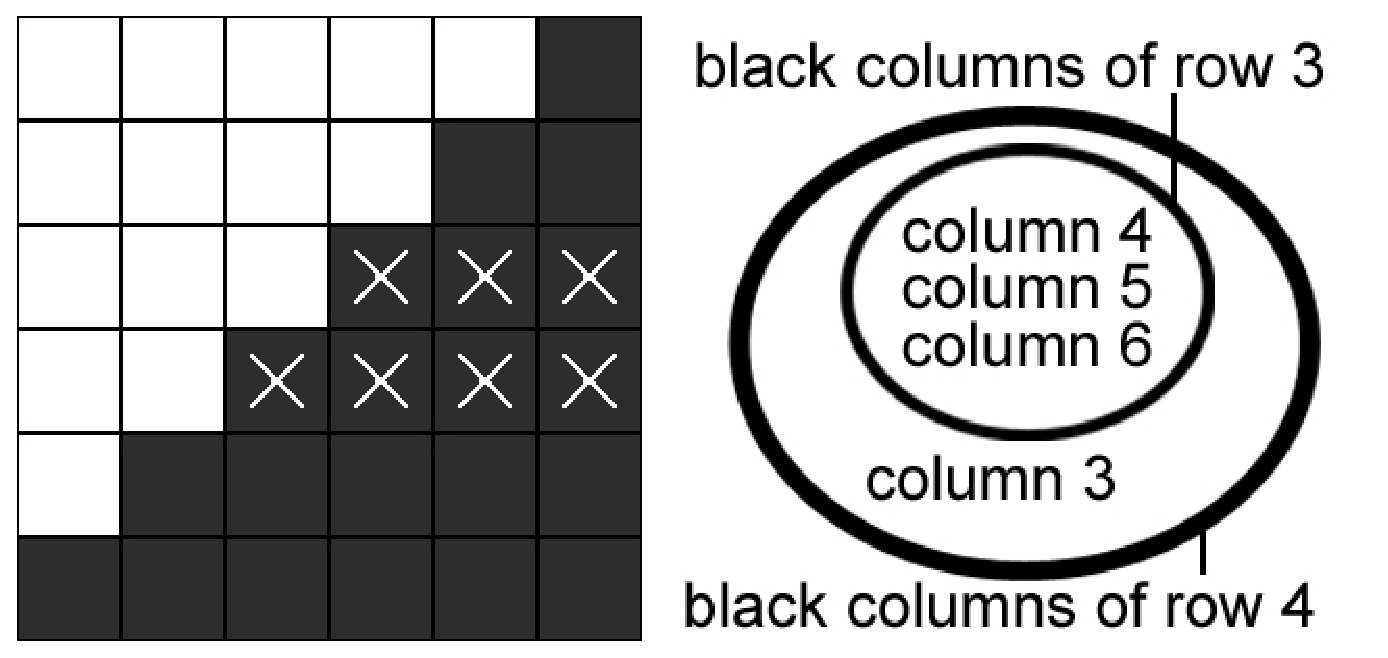
\includegraphics[height=4cm]{monotonicity_example_good}
\caption{A pattern that follows the Monotonicity Property.}
\end{figure}

\begin{figure}[h]
\centering
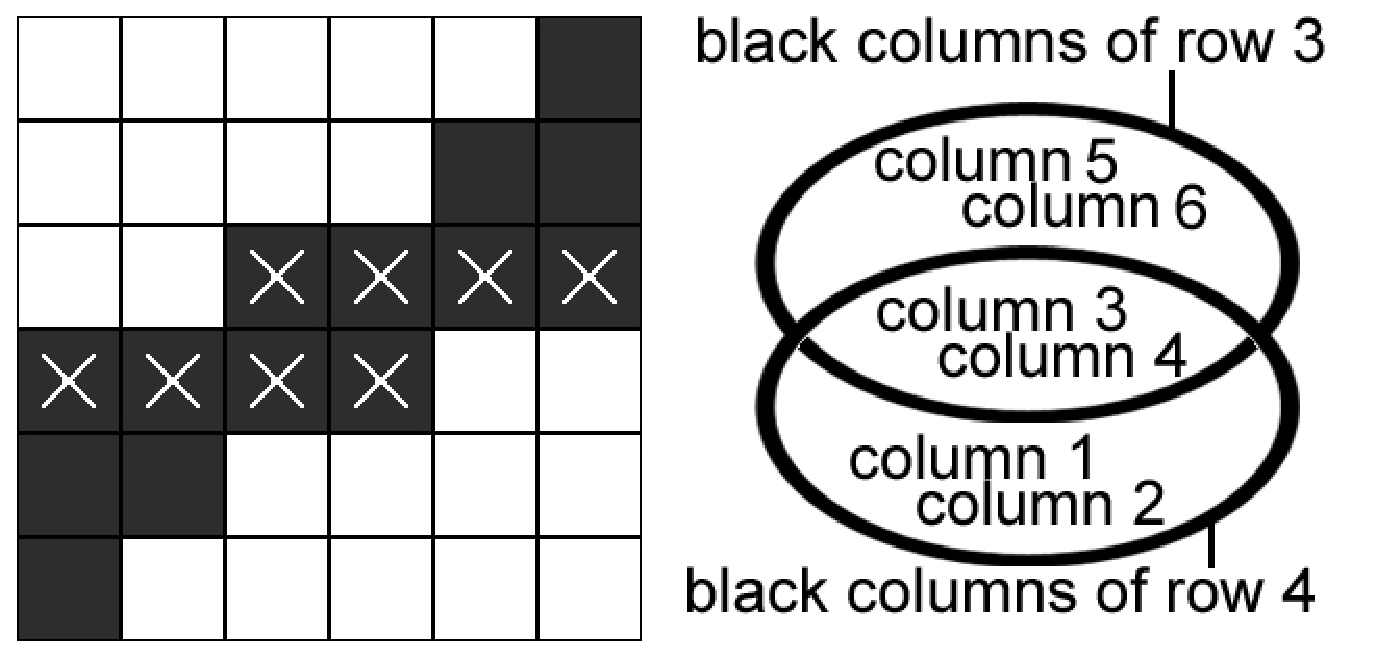
\includegraphics[height=4cm]{monotonicity_example_bad}
\caption{A pattern that does not follow the Monotonicity Property.}
\end{figure}

\end{theorem}

This theorem will allow us to order the columns and rows of a strip-rule pattern P in a non-decreasing sequence regarding the number of black cells. Once the $i$-th black cell is achieved in the sequence, that $i$-th cell will remain black until the end of the sequence.


Since Theorem 3.1 of \cite{ACJKLW07} is not proven in their conference version,
we include a proof for the sake of completeness.
\begin{proof}

Let's begin our proof by verifying that items (i) and (ii) of the Monotonicity Property are equivalent.


I.) $(i) \leftrightarrow (ii)$

Let's start by proving that $\neg (i) \rightarrow \neg (ii)$. Suppose (i) does not hold. Then, given $c \in \{black, white\}$, there are two rows A and B , $A \neq B$, of $P$ that do no follow the property mentioned above. Without loss of generality, let's say $c = black$. Since one set is not contained into each other, it must be the case where both sets contains a element that the other set does not have.

This implies that both of the following are true at the same time:

\begin{enumerate}%[(a)]
\item There is a column that has a black cell on row A and a white cell on row B.
\item There is a column that has a black cell on row B and a white cell on row A.
\end{enumerate}

For reference, let's call this case a checkerboard case.

\begin{figure}[h]
\centering
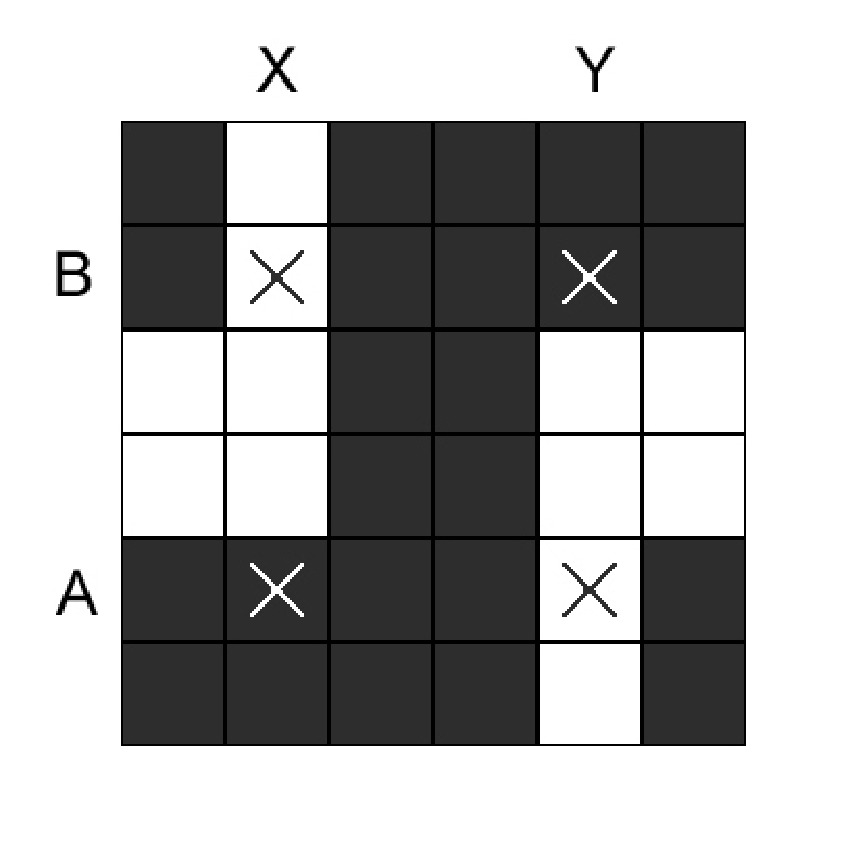
\includegraphics[height=4cm]{checkerboard_example}
\caption{Example of a checkerboard case, where (i) does not hold.}
\end{figure}

Let X and Y be one of those columns described in (a) and (b) respectively. The set of rows where black is present in X has A as one of its rows and the set of rows where black is present in Y has B as one of its rows. Hence, those sets are not contained into each other. As a result, (ii) does not hold. Thus it must be true that (ii) implies (i). ($(ii) \rightarrow (i)$)

The same argument can be made with the roles of rows and columns switched, leading to a conclusion that (i) implies (ii). ($(i) \rightarrow (ii)$) Then it must be true that (i) and (ii) are equivalent.


Let's continue with the equivalence of $P$ being a strip-rule pattern and the Monotonicity property. Let's divide the proof into two steps:

\begin{itemize}

\item ($P$ is a strip-rule pattern) $\rightarrow$ (Monotonicity Property)

We will prove that $\neg$(Monotonicity Property) $\rightarrow$ $\neg$($P$ is a strip-rule pattern). Suppose the Monotonicity property does not hold true. By contradiction, suppose that $P$ is a strip-rule pattern and let $S$ be a strip-rule RRL of size $n$ that generates $P$ such that $S = (s_{1},s_{2},\cdots,s_{n})$.

Since the Monotonicity property does not hold true, the same argument as before for the checkerboard case can be made. Let $s_{i}$ be the last rule of $S$ that includes one of the rows or columns of the checkerboard case. Since $s_{i}$ is the last rule that they appear, no other rule after $s_{i}$ could have changed the intersection of the rows ${A,B}$ and columns ${X,Y}$ of the checkerboard case. Then, because of $s_{i}$, either A, B, X or Y must have same color cells in the checkerboard. However, if that happens, the checkerboard case does not hold anymore - a contradiction. Hence, $P$ is not a strip-rule pattern and ($P$ is a strip-rule pattern) $\rightarrow$ (Monotonicity Property) must hold true.

\item (Monotonicity Property) $\rightarrow$ ($P$ is a strip-rule pattern)


Suppose that the Monotonicity property holds. By contradiction, suppose that $P$ is not a strip-rule pattern.
By \ref{theorem_pick_up_sticks}, the MPUS algorithm will not stop with a all-gray grid. Then it must have been stuck at a grid with no pseudo-monochromatic row or column.

Let A be the row with the largest number of cells colored black. Since this row is not monochromatic, there must be a column Y which intersection with A is a white cell. Y must also not be pseudo-monochromatic. So there must a row B that intersects Y with a black cell. Since B has a black cell in a column that A does not have, than it must be true that the black columns of A are a subset of the black columns of B because of the Monotonicity property. Note also that those sets must not be equal.

Hence, the number of black cells in B is higher than A, a contradiction. As a conclusion, (Monotonicity Property) $\rightarrow$ ($P$ is a strip-rule pattern) must hold, which concludes our proof.
\end{itemize}

In conclusion,  have shown that patterns generated by RRLs and patterns
that are satisfy monotonicity are equivalent.
This allows us to label the row and column classes by the number of black
cells they contain.
For example, every row that has exactly 4 black cells will be identical and
can be grouped into the class named $R_4$.
Our algorithm uses this principle to organize and determine the order of
classes to be removed.
The fact that RRL patterns have all the properties of monotonicity will
helpful is number of following proofs.
\qed
\end{proof}
